\chapter{Les atomes de Rydberg circulaires en interaction : vers un simulateur quantique}
\label{chapter:circsim}

%Intro : pourquoi envisager les Rydberg circulaires comme plateforme de simulation ?
\noindent La bonne compréhension des interactions entre atomes de Rydberg sphériques permet d'imaginer leur utilisation comme plateforme de simulation quantique.
%Les simulations menées par Thanh Long Nguyen \cite{PHD_NGUYEN} montrent la difficulté de la préparation déterministe d'un ensemble d'atomes de Rybderg adapté à cette fin.
Un premier obstacle majeur s'oppose à cette idée.
La préparation d'une chaîne régulière d'atomes de Rydberg dans le niveau $\mathrm{60S}$ en s'appuyant sur le mécanisme d'excitation facilitée paraît difficile \cite{PHD_NGUYEN}.

Nous présentons ici une proposition de simulateur quantique à partir d'atomes de Rydberg circulaires piégés par laser.
Cette proposition est formulée en détail dans la thèse de Thanh Long Nguyen \cite{PHD_NGUYEN}.
L'article \cite{ENS_PRE_CIRCSIM} en reprend les points essentiels.

Le simulateur proposé repose sur les interactions entre atomes de Rydberg circulaires.
Nous dirons quelques mots de celles-ci en présence d'un champ électrique et d'un champ magnétique externe, en complément de \ref{subsec:interac50C_I}.
Ces interactions permettent de simuler le hamiltonien \og XXZ \fg{} d'une chaîne de spins $1/2$, que nous présenterons.
Nous terminerons ce chapitre avec une discussion des points techniques nécessaires à la réalisation d'un tel simulateur : le piégeage laser des atomes de Rydberg circulaires, l'allongement de leur durée de vie par inhibition de l'émission spontanée et la préparation déterministe d'une chaîne de tels atomes.


\section{Les interactions dipôle-dipôle entre atomes de Rydberg circulaires}
\noindent Les interactions dipôle-dipôle entre atomes de Rydberg circulaires sont au c\oe ur de notre proposition de simulateur.
Comme nous l'avons mentionné en \ref{subsec:interac50C_I}, la présence d'un champ électrique externe permet de fixer un axe de quantification, et donc de fixer l'orientation des orbites de grand moment cinétique.
Dans la présente discussion, nous considérerons que les atomes de Rydberg circulaires sont placés sur un axe $Ox$, perpendiculaire au champ directeur selon $Oz$, tels que représentés en figure \eqref{fig:double_torus}.

%\subsection{La structure des niveaux atomiques et des niveaux de paire près des circulaires}
\subsection{Les niveaux circulaires en présence de champs électrique et magnétique}
\noindent En présence d'un champ électrique, les niveaux à grand moment cinétique d'une même multiplicité voient leur dégénérescence partiellement levée.
Le diagramme d'énergie de ces niveaux est représenté en figure (\ref{fig:ener_StarknC_nCnC}a)).
Le niveau circulaire est noté $\ket{\mathrm{nC}}$ et les deux niveaux \og elliptiques \fg{} voisins sont notés $\ket{\mathrm{nE^{\pm}}} = \ket{n,m=n-2,k=\pm1}$.
De la même façon, les niveaux de $m=n-3$ sont notés $\ket{\mathrm{nEE^0}} = \ket{n,m=n-3,k=0}$ et $\ket{\mathrm{nEE^{\pm}}} = \ket{n,m=n-3,k=\pm 2}$.
%
\begin{figure}[!h]
\centering
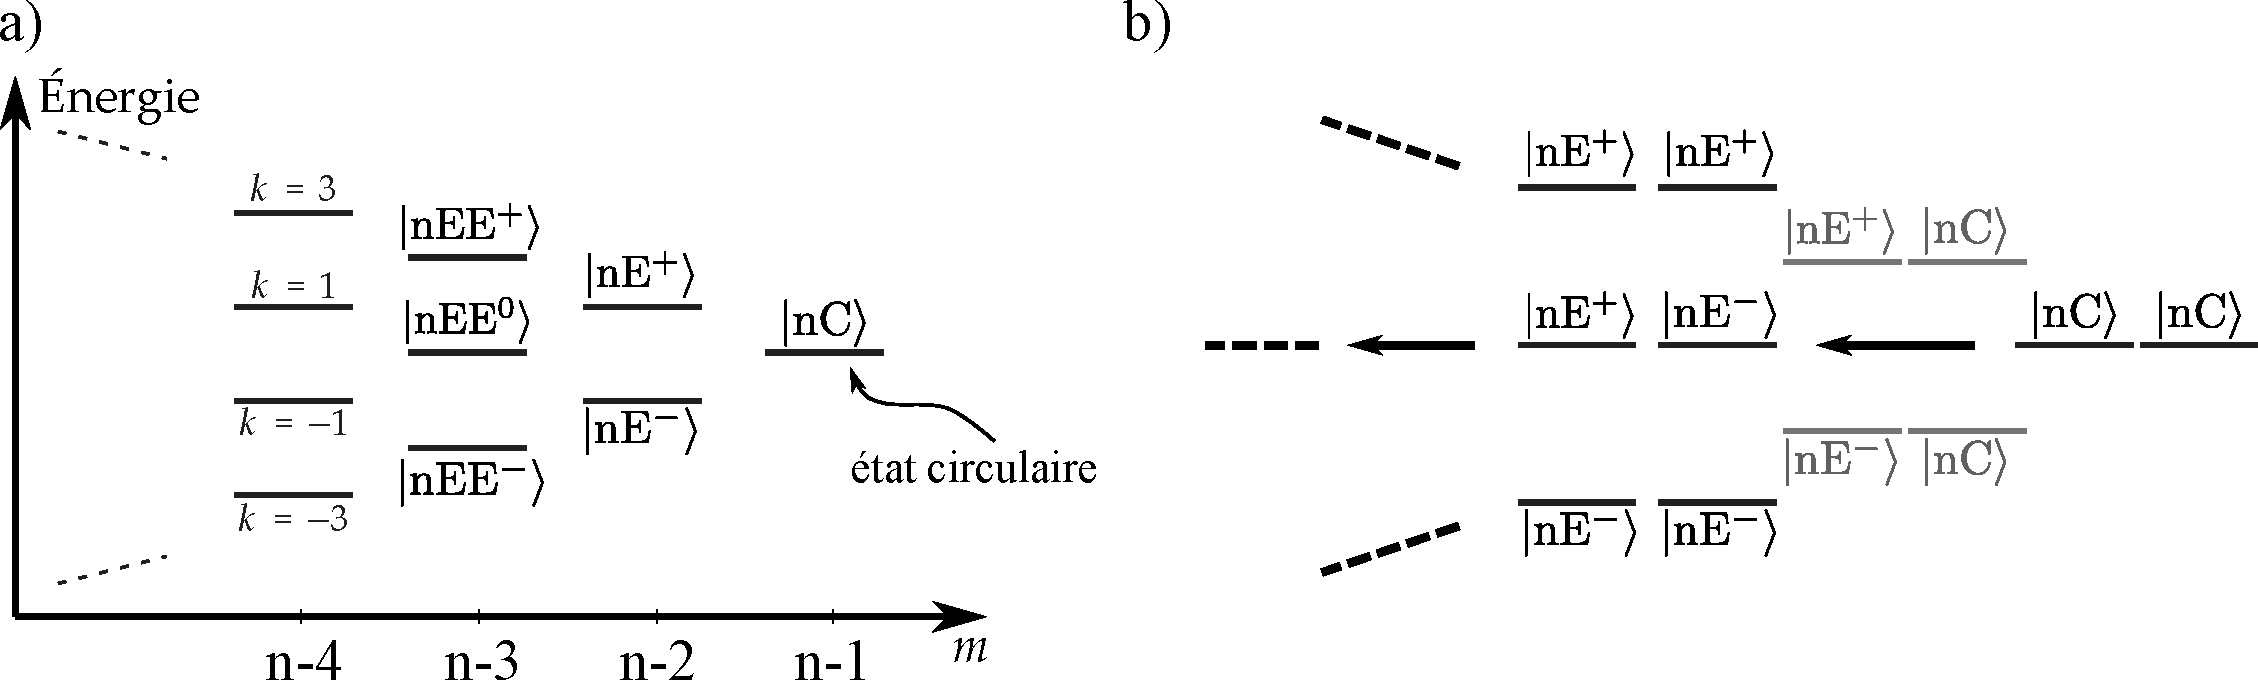
\includegraphics[width=\linewidth]{figures/circsim/diagram_nC_nCnC}
\caption[Diagammre d'énergie des niveaux proches du $\mathrm{50C}$]{
\textbf{a)} Diagramme d'énergie des niveaux proches de $\mathrm{nC}$, en présence d'un champ électrique.
\textbf{b)} Diagramme d'énergie des niveaux de paire proches de $\ket{\mathrm{nC}}\ket{\mathrm{nC}}$ en présence d'un champ électrique.
Le champ électrique est dirigé selon $Oz$, perpendiculaire au vecteur qui sépare les deux atomes de la paire,  dirigé selon $Ox$.
}
\label{fig:ener_StarknC_nCnC}
\end{figure}

%\noindent Il est utile de rappeler ici la forme analytique de l'énergie des niveaux proches du circulaire en présence d'un champ électrique $\vec{F}$, tirée de l'équation \eqref{eq:Stark_circular} :
%%
%\begin{equation}
%\label{eq:Stark_nC_explicit}
%\begin{aligned}
%E_{\mathrm{nC}} &= -\frac{1}{2n^2} - \frac{1}{16}n^4(8n^2+18n+10)|\vec{F}|^2\\
%&=-\frac{1}{2n^2}+\alpha_{\mathrm{nC}}|\vec{F}|^2 ,\\
%E_{\mathrm{nE^{\pm}}} &= -\frac{1}{2n^2} \pm \frac{3n}{2}|\vec{F}| -  \frac{1}{16}n^4(8n^2+36n-20)|\vec{F}|^2 \\
%&=-\frac{1}{2n^2} \pm \frac{3n}{2} +\alpha_{\mathrm{nE^{\pm}}}|\vec{F}|^2 ,
%\end{aligned}
%\end{equation}
%%
%où les coefficients $\alpha$ d'effet Stark quadratique sont introduits pour simplifier l'écriture.

Il s'agit maintenant de comprendre quelle forme prend l'interaction dipôle-dipôle dans le cas présent.
Replaçons nous dans le cas de deux atomes séparés d'une distance $r$.
En \ref{sec:interacting_rydbergs} nous avions exprimé, en l'absence de champ électrique extérieur, le hamiltonien de couplage dans la base des harmoniques sphériques (cf. équation \eqref{eq:Vdd_rr1r2}).
De plus, l'axe de quantification était alors déterminé par le vecteur séparant la paire d'atomes en interaction.
Ici au contraire, l'axe de quantification est déterminé par le champ électrique extérieur, selon $Oz$ donc, et le vecteur séparant les atomes sont situés sur l'axe $Ox$, à des positions $\vec{r_1},\vec{r_2}$ respectivement.
Le hamiltonien d'interaction dipôle-dipôle prend alors la forme
\begin{equation}
\label{eq:dipdip_nC}
\hat{V}_{dd} = -\frac{q^2\hat{r_1} \hat{r_2}}{3\epsilon_0 r^3}
\left[ Y_1^0 Y_1^0 + \frac{1}{2} \left( Y_1^{+1}Y_1^{-1} + Y_1^{-1}Y_1^{+1} \right)
- \frac{3}{2} \left(  Y_1^{+1}Y_1^{+1} + Y_1^{-1}Y_1^{-1} \right) \right],
\end{equation}
où les $Y_l^m$ sont les harmoniques sphériques.
On remarque ici que le moment magnétique total de la paire atomique n'est plus nécessairement conservé par l'interaction dipôle-dipôle.
Ainsi le niveau de paire $\ket{\mathrm{nC},\mathrm{nC}}$ se trouve couplé de façon quasi résonante avec le niveau de paire $\ket{\mathrm{nE^+},\mathrm{nE^-}}$, lui-même couplé aux niveaux de paire $\ket{\mathrm{nEE^+},\mathrm{nEE^-}}$ et $\ket{\mathrm{nEE^0},\mathrm{nEE^0}}$, et ainsi de suite.
La figure (\ref{fig:ener_StarknC_nCnC} b) représente les niveaux de paire proches du niveau $\ket{\mathrm{nC},\mathrm{nC}}$ en présence d'un champ électrique.

Ces couplages quasi résonants, dès lors que la distance entre les atomes est suffisamment petite, perturbent le niveau $\ket{\mathrm{nC,nC}}$ en le mélangeant aux niveaux de paires d'énergie suffisamment proche.
C'est ce que nous avions vu en \ref{subsec:interac50C_I} : en figure \eqref{fig:VdW_50C50C_1Vcm}, lorsque les deux atomes de la paire sont plus proches que $\SI{10}{\um}$, l'état propre du hamiltonien complet s'éloigne du niveau non perturbé $\ket{\mathrm{50C,50C}}$.
Cet effet de mélange a plusieurs conséquences néfastes.
Tout d'abord, l'interaction dipôle-dipôle ne peut plus être simplement approximée par un déplacement d'énergie en $1/r^6$ entre deux atomes dans un niveau de paire $\ket{n,k,m}\ket{n,k,m}$.
De plus, le mélange avec les niveaux elliptiques réduit le temps de vie du niveau de paire à deux atomes circulaires.
En effet, les niveaux elliptiques peuvent être deséxcités par des transitions $\pi$ vers la multiplicité inférieure alors que le niveau circulaire ne peut être deséxcité que par une transition $\sigma^+$.
Or le dispositif d'inhibition de l'émission spontanée que nous proposons, qui sera discuté en \ref{subsec:inhibition}, ne peut inhiber que l'émission spontanée $\sigma^+$.
Ainsi donc, le gain de temps de vie permis par ce dispositif est perdu dès lors que des transitions $\pi$ sont accessibles.

Afin de contourner cette difficulté, il faut trouver un moyen de lever la dégénérescence des niveaux de paire non perturbés représentés en figure (\ref{fig:ener_StarknC_nCnC} b).
Deux paramètres sont à notre disposition pour ce faire.
Le premier est la valeur du champ électrique.
Les niveaux de paire non perturbés sont d'autant plus distants en énergie que le champ électrique est élevé.
Cependant, la variation du champ électrique nous servira à faire varier l'interaction elle-même comme nous l'expliquerons en \ref{subsec:tunability}.
Le second moyen dont nous disposons est l'imposition d'un champ magnétique extérieur $B_z$, orienté selon $Oz$, qui déplacera les niveaux par effet Zeeman.

Le hamiltonien Zeeman pour un état circulaire prend alors la forme%\footnote{
%on néglige le spin de l'électron
%}
\begin{equation}
\label{eq:H_Zeeman}
\hat{H}_Z = \mu_B g_l~\hat{\vec{L}}\cdot\vec{B} = \mu_B g_l\hat{L}_zB_z,
%\frac{\mu_B g_l}{\hbar}~\hat{\vec{L}}\cdot\vec{B} = \frac{\mu_B g_l}{\hbar}\hat{L}_zB_z,
\end{equation}
où $\mu_B$ est le magnéton de Bohr et $g_l$ le facteur de Landé pour le nombre quantique orbital $l$.
Dans la mesure où l'on néglige le spin de l'électron, qui est très petit devant $l$ ($s=1/2 \ll l\simeq 50$), le facteur de Landé peut être approximé à $g_l \simeq -1$.
Ce hamiltonien conserve le nombre quantique magnétique $m$, qui n'est autre que la valeur propre de l'opérateur $\hat{L_z}$\footnote{
Si le champ magnétique avait des composantes non nulles selon $Ox$ et $Oy$, celles-ci coupleraient des états de $m$ différents.}.
Tant que le champ magnétique $B_z$ reste suffisamment petit, l'effet Zeeman agit comme une perturbation au premier ordre du hamiltonien \eqref{eq:hamilt_Stark} de l'atome dans un champ électrique.
La seule conséquence de l'effet Zeeman sur le niveau $\ket{n,m,k}$ sera un déplacement d'énergie
\begin{equation}
\label{eq:Zeeman_shift}
\Delta E_Z (n,m,k) = \braket{n,m,k|g_l \hat{L}_z | n,m,k}\cdot \mu_B B_z \simeq m\cdot \mu_B B_z = \Delta E_Z (m).
\end{equation}
Le niveau de paire $\ket{n,m,k ; n,m',k'}$ sera déplacé de la somme du déplacement d'énergie de $\ket{n,m,k}$ et $\ket{n,m',k'}$, soit $(m+m')\mu_B B_z$.

En tenant compte de l'effet Stark (cf. équation \eqref{eq:Stark_circular}) et de l'effet Zeeman perturbatif, on obtient les énergies suivantes pour les niveaux circulaires et elliptiques de la multiplicité $n$ :
\begin{equation}
\label{eq:ener_nC_ZeeStark}
\begin{aligned}
E_{\mathrm{nC}}/2E_I &= -\frac{1}{2n^2} - \frac{1}{16}n^4(8n^2+18n+10)|\vec{F}|^2 \left(\frac{ea_0}{2E_I} \right)^2 + (n-1)\mu_B B_z \\
&= -\frac{1}{2n^2} - \alpha_{\mathrm{nC}}|\vec{F}|^2 + (n-1)\mu_B B_z ,\\
E_{\mathrm{nE^{\pm}}}/2E_I &= -\frac{1}{2n^2} \pm \frac{3n}{2}|\vec{F}|\frac{ea_0}{2E_I} - \frac{1}{16}n^4(8n^2+36n-20)|\vec{F}|^2\left(\frac{ea_0}{2E_I} \right)^2 + (n-2)\mu_B B_z \\
&= -\frac{1}{2n^2} \pm \frac{ea_0}{2E_I}\frac{3n}{2}|\vec{F}| +\alpha_{\mathrm{nE^{\pm}}}|\vec{F}|^2 + (n-2)\mu_B B_z,
\end{aligned}
\end{equation}
où les coefficients $\alpha$ d'effet Stark quadratique sont introduits pour simplifier l'écriture.

Appliquons les équations \eqref{eq:ener_nC_ZeeStark} à l'exemple des états de paire non perturbés $\ket{\mathrm{50C,50C}}$ et $\ket{\mathrm{50E^+,50E^-}}$.
Dans les conditions du paragraphe \ref{subsec:interac50C_I}, c'est-à-dire sous $\SI{1}{\V/cm}$ et sans champ magnétique, la distance en énergie entre ces deux états de paire est de $\Delta_E = h\times\SI{169}{\kHz}$.
Si l'on ajoute un champ magnétique $B_z$ de $\SI{10}{\gauss}=\SI{1}{\milli\tesla}$, la distance en énergie devient $\Delta E = h\times \SI{28.17}{\MHz}$, soit presque $\SI{200}{}$ fois plus.
Un faible champ magnétique nous permet ainsi de lever la dégénérescence entre les niveaux de  paire voisins de $\ket{\mathrm{nC,nC}}$.

\subsection{L'interaction circulaire-circulaire en présence de champs électrique et magnétique extérieurs}
\noindent Dans les condition que nous venons d'établir il nous est possible de calculer l'interaction dipôle-dipôle entre deux atomes circulaires, tout en limitant la perturbation de ces niveaux qui serait due à un couplage résonant.
Ce calcul s'effectue de la même façon qu'en \ref{sec:interacting_rydbergs}, en diagonalisant le hamiltonien complet de la paire atomique\footnote{
La même méthode permet tout aussi bien de calculer l'interaction entre deux atomes dans des niveaux différents, de même qu'en \ref{sec:interacting_rydbergs}.
}.
Ce hamiltonien complet s'écrit
\begin{equation}
\label{eq:hamilt_Vdd_ZeeStark}
\begin{aligned}
\hat{H} &= \hat{H}_1 + \hat{H}_2 + \hat{V}_{dd}(\vec{r}) \\
 &= \hat{H}_{0,1} + \hat{H}_{0,2} + \hat{H}_{S,1} + \hat{H}_{S,2} + \hat{H}_{Z,1} + \hat{H}_{Z,2} + \hat{V}_{dd}(\vec{r}),
\end{aligned}
\end{equation}
où $\hat{H}_{0,i},\hat{H}_{S,i},\hat{H}_{Z,i}$ sont respectivement les hamiltoniens libre, Stark et Zeeman de l'atome $i$ et $\hat{H}_i$ le hamiltonien total de l'atome $i$ isolé.

Nous pouvons, ici encore, écrire l'interaction entre un atome dans le niveau $\mathrm{nC}$ et un atome dans le niveau $\mathrm{n'C}$ comme un hamiltonien effectif
\begin{equation}
\label{eq:Veff_nCn'C}
V_{eff}/h = \left(\begin{array}{cc}
C_{\mathrm{nC},\mathrm{n'C}} & A_{\mathrm{nC},\mathrm{n'C}} \\
A_{\mathrm{nC},\mathrm{n'C}} & C_{\mathrm{nC},\mathrm{n'C}},
\end{array} \right)
\end{equation}
où $C_{\mathrm{nC},\mathrm{n'C}}$ et $A_{\mathrm{nC},\mathrm{n'C}}$ sont respectivement les termes d'interaction directe et d'échange entre les niveaux $\mathrm{nC}$ et $\mathrm{n'C}$.
De manière générale, ces termes se décomposent en une composante \og van der Waals \fg{} en $1/r^6$ et une composante de couplage direct en $1/r^3$.
De plus, ils dépendent désormais fortement des champs électrique et magnétique imposés.

Reprenons l'exemple d'une paire $\ket{\mathrm{50C,50C}}$.
Les deux atomes étant dans le même état, l'interaction se limitera aux termes diagonaux du hamiltonien \eqref{eq:Veff_nCn'C} et aucune interaction d'échange n'aura lieu.
Dans le paragraphe \ref{subsec:interac50C_I}, sans champ magnétique extérieur et sous $\SI{1}{\V/\cm}$, le niveau de paire se mélangeait dès que la distance entre les deux atomes était inférieure à $\SI{10}{\um}$.
Le résultat de ce calcul est à nouveau présenté en figure (\ref{fig:VdW_50C50C_1Vcm_10G} a).
En refaisant le calcul avec un champ magnétique $B_z=\SI{10}{\gauss}$, on obtient la courbe d'énergie présentée en figure (\ref{fig:VdW_50C50C_1Vcm_10G} b).
%
\begin{figure}[h]
\centering
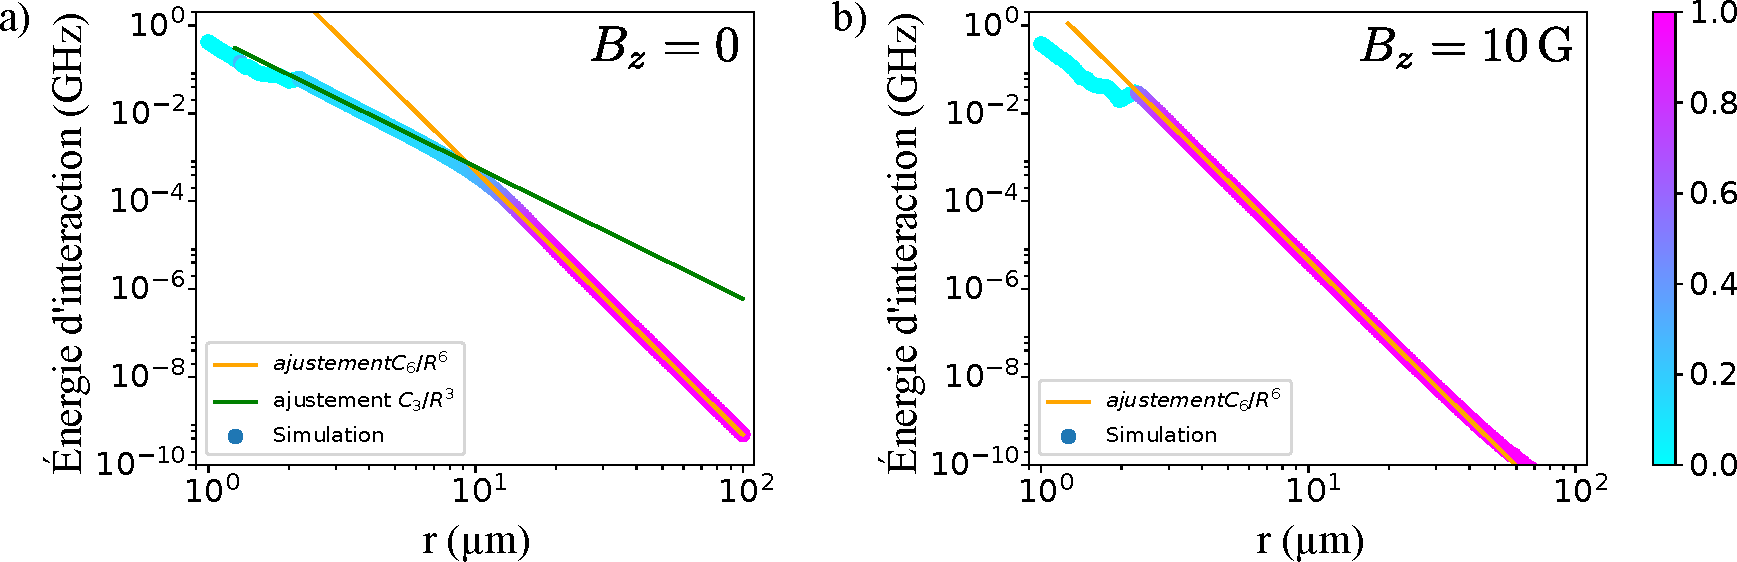
\includegraphics[width=\linewidth]{figures/circsim/VdW_50C50C_1Vcm_0_10G}
\caption[Interaction dipolaire 50C-50C en présence d'un champ magnétique]{
Déplacement en énergie de la paire 50C-50C par interaction dipolaire.
Les deux atomes sont placés côte à côte sur l'axe $Ox$, sous un champ électrique de $\SIvv{1}{\V / \cm}$ selon l'axe $Oz$. L'échelle de couleur représente le carré de la projection sur l'état non perturbé $\ket{50\text{C},50\text{C}}$ de l'état propre du hamiltonien qui le suit adiabatiquement.
\textbf{a)} Sans champ magnétique extérieur et \textbf{b)} avec un champ magnétique $B_z = \SI{10}{\gauss}$ selon $Oz$.
}
\label{fig:VdW_50C50C_1Vcm_10G}
\end{figure}
%
Alors qu'en l'absence de champ magnétique le niveau de paire circulaire-circulaire était perturbé dès que la distance entre les deux atomes était inférieure à $\SI{10}{\um}$, un champ magnétique de $\SI{10}{\gauss}$ selon $Oz$ permet d'éviter cet effet.
L'énergie d'interaction évolue ainsi en $1/r^6$ pour les distances supérieures à $\SI{2}{\um}$.
Cependant, l'interaction est rendue moins forte.
En effet, un ajustement en $1/r^6$ donne un coefficient de van der Waals $C_{6,\mathrm{50C-50C}}(\SI{10}{\gauss}) = \SI{4.45}{\GHz\raiseto{6}\um}$ au lieu de $\SI{489.18}{\GHz\raiseto{6}\um}$ en champ magnétique nul.
Cela s'explique par le fait que le couplage dipolaire second de ordre varie comme l'inverse des distances en énergie entre le niveau de paire considéré et les niveaux médiateurs du couplage.
Le champ magnétique ayant pour effet de déplacer les niveaux de paire de façon à supprimer les couplages quasi résonants, il s'en suit que les distance en énergie entre niveaux de paire sont augmentées et l'interaction d'autant diminuée.

En raison de cette réduction du coefficient de van der Waals $C_6$, l'interaction à grande distance n'est plus dominée par les couplages de second ordre en $1/r^6$, mais par des couplages de premier ordre en $1/r^3$.
Il devient donc nécessaire, afin de bien décrire l'évolution de l'énergie d'interaction à grande distance, de l'ajuster à une forme mixte en $C_3/r^3 + C_6/r^6$.
Un tel ajustement est présenté en figure (\ref{fig:VdW_50C50C_1Vcm_10G} b).
Il donne les coefficients $C_{6,\mathrm{50C-50C}}(\SI{10}{\gauss}) = \SI{4.23}{\GHz\raiseto{6}\um}$ et $C_{3,\mathrm{50C-50C}}(\SI{10}{\gauss}) = \SI{1.02e-5}{\GHz\raiseto{3}\um}$.
Dans les discussions qui suivent, nous nous limiterons à des distances inter-atomiques de l'ordre de $\SI{5}{\um}$, et omettrons par conséquent d'indiquer cette composante en $1/r^3$ de l'interaction, qui n'est importante qu'à grande distance.

Dans le cas d'une paire d'atomes dans l'état $\ket{\mathrm{nC,n'C}}$ avec $n'\neq n$, une interaction d'échange décrite par le coefficient $A_{\mathrm{nC},\mathrm{n'C}}$ aura lieu, en plus de l'interaction directe décrite par le coefficient $C_{\mathrm{nC},\mathrm{n'C}}$.
Celle-ci permet d'envisager la simulation d'un ensemble de spins $1/2$.

\section{Le hamiltonien $XXZ$ simulé}
\newcommand{\CnCnC}{C_{\mathrm{nC},\mathrm{nC}}}
\newcommand{\CnpCnpC}{C_{\mathrm{n'C},\mathrm{n'C}}}
\newcommand{\CnCnpC}{C_{\mathrm{nC},\mathrm{n'C}}}
\newcommand{\AnCnpC}{A_{\mathrm{nC},\mathrm{n'C}}}

	\subsection{Équivalence avec une paire de spins $1/2$}
\noindent Étant donné que nous souhaitons simuler une chaîne de spins $1/2$, il nous faut étendre la base des états accessibles.
L'état d'un spin $1/2$ est décrit sur la base $\{\ket{\uparrow},\ket{\downarrow}\}$ et l'état d'une paire de spins $1/2$ est décrit sur la base $\{ \ket{\uparrow \uparrow},\ket{\uparrow \downarrow}, \ket{\downarrow\uparrow}, \ket{\downarrow\downarrow} \}$.
Ainsi en encodant le spin sur des états de Rydberg circulaires par l'équivalence $\ket{\uparrow} = \ket{\mathrm{nC}} , \ket{\downarrow} = \ket{\mathrm{n'C}}$, le hamiltonien d'interaction de la paire de spin doit être étendu à la base 
$\{ \ket{\mathrm{nC},\mathrm{nC}},\ket{\mathrm{nC},\mathrm{n'C}}, \ket{\mathrm{n'C},\mathrm{nC}}, \ket{\mathrm{n'C},\mathrm{n'C}} \}$.
Sur cette base, le hamiltonien d'interaction prend la forme
\begin{equation}
\label{eq:V_eff_nCnC_n'Cn'c}
\hat{V}_{eff}/h = \bordermatrix{
~ 	&\ket{\mathrm{nC},\mathrm{nC}} 	&\ket{\mathrm{nC},\mathrm{n'C}} 
&\ket{\mathrm{n'C},\mathrm{nC}} &\ket{\mathrm{n'C},\mathrm{n'C}} \cr
	\bra{\mathrm{nC},\mathrm{nC}}	& C_{\mathrm{nC},\mathrm{nC}} & 0 & 0 & 0 \cr 
	\bra{\mathrm{nC},\mathrm{n'C}} 	& 0 & C_{\mathrm{nC},\mathrm{n'C}} & A_{\mathrm{nC},\mathrm{n'C}} & 0 \cr
	\bra{\mathrm{n'C},\mathrm{nC}} 	& 0 & A_{\mathrm{nC},\mathrm{n'C}} & C_{\mathrm{nC},\mathrm{n'C}} & 0 \cr
	\bra{\mathrm{n'C},\mathrm{n'C}} & 0 & 0 &  0	& C_{\mathrm{n'C},\mathrm{n'C}}\cr
	}
\end{equation}


Nous souhaitons écrire ce hamiltonien sur la base des opérateurs de spin.
Pour chacun des spins, ces opérateurs sont décrits sur la base de l'identité et des matrices de Pauli $\{\mathbbm{1},\sigma^\alpha \}_{\alpha=x,y,z}$.
Afin d'agir sur l'espace produit tensoriel de deux spins, il nous faut définir les opérateurs suivants
\begin{equation}
\label{eq:Pauli_tensor_space}
\begin{aligned}
\sigma_1^\alpha &= \sigma^\alpha \otimes \mathbbm{1} \\
\sigma_2^\alpha &= \mathbbm{1} \otimes \sigma^\alpha
\end{aligned},
\end{equation}
où l'indice $1$ ou $2$ indique sur quel atome agit l'opérateur.
La famille formée par les produits matriciels deux à deux de ces opérateurs $\mathbbm{1}$\footnote{
Nous omettons délibérément la dimension de l'espace sur lequel agit l'opérateur d'identité. Celui-ci devrait en toute rigueur s'écrire $\mathbbm{1}\otimes \mathbbm{1} = \mathbbm{1}^{\otimes 2}$.
} et $\sigma_i^\alpha$ permet de générer tous les opérateurs agissant sur la paire de spins.
Nous pouvons ainsi réécrire le hamiltonien d'interaction \eqref{eq:V_eff_nCnC_n'Cn'c} sous la forme
%
\begin{equation}
\label{eq:Veff_2at_Pauli}
\begin{aligned}
\hat{V}_{eff}/h &= \delta E~\mathbbm{1}
+ \frac{\delta\zeta}{2}\left( \sigma_1^z + \sigma_2^z \right)
+ J_z\left( \sigma_1^z \sigma_2^z \right)
+ J \left( \sigma_1^x \sigma_2^x + \sigma_1^y \sigma_2^y \right) \\
&= \left( \begin{array}{cccc}
\delta E + \delta \zeta + J_z & 0 & 0 & 0 \\
0 & \delta E - J_z & 2J & 0 \\
0 & 2J & \delta E - J_z & 0 \\
0 & 0 & 0 & \delta E - \delta \zeta + J_z \\
\end{array} \right),
\end{aligned}
\end{equation}
%
où l'on identifie :
%
\begin{equation}
\label{eq:ident_XXZ}
\left\{
\begin{aligned}
\delta E &= \left( \CnCnC + 2\CnCnpC + \CnpCnpC \right)/4, \\
\delta \zeta &= \left( \CnCnC - \CnpCnpC \right)/2, \\
J_z &= \left( \CnCnC - 2\CnCnpC + \CnpCnpC \right)/4, \\
J &= \AnCnpC /2~.
\end{aligned} \right.
\end{equation}
%
Notons que le terme $\delta E \mathbbm{1}$ ne fait que redéfinir l'origine des énergies, et peut donc être ignoré.
Le hamiltonien d'interaction de la paire devient ainsi
\begin{equation}
\label{eq:XXZint_2atoms}
\hat{V}_{eff,\text{2 atomes}}/h = \frac{\delta\zeta}{2}\left( \sigma_1^z + \sigma_2^z \right)
+ J_z\left( \sigma_1^z \sigma_2^z \right)
+ J \left( \sigma_1^x \sigma_2^x + \sigma_1^y \sigma_2^y \right).
\end{equation}
%connu comme \og hamiltonien XXZ \fg{}.

	\subsection{Extension à une chaîne de $N$ atomes et habillage microonde}
\noindent Le hamiltonien d'interaction à deux atomes s'étend facilement à une chaîne de $N$ atomes régulièrement espacés d'un distance $r$ et numérotés de $1$ à $N$.
Nous pouvons ici négliger les interactions au-delà du premier voisin.
En effet, dès lors que les termes d'interaction évoluent en $1/r^6$, la contribution d'un second voisin est $\SI{64}{}$ fois plus petite que celle des premiers voisins.
Le hamiltonien d'interaction d'une telle chaîne de spin s'écrit alors, en généralisant le hamiltonien à deux atomes \eqref{eq:XXZint_2atoms},
%
\begin{equation}
\label{eq:XXZint_Natoms}
\hat{V}_{eff,\text{N}}/h =
\frac{\delta\zeta}{2} \left( \sigma_1^z + \sigma_N^z \right)
+ \delta\zeta \sum_{i=2}^{N-1} \sigma_i^z
+ J_z \sum_{i=1}^{N-1} \sigma_i^z \sigma_{i+1}^z
+ J \sum_{i=1}^{N-1} \left( \sigma_i^x \sigma_{i+1}^x + \sigma_i^y \sigma_{i+1}^y \right) ,
\end{equation}
%
où les opérateurs de spin $\sigma_i^\alpha$ agissant sur l'atome $i$ sont définis par
%
\begin{equation}
\label{eq:Pauli_Natoms}
\sigma_i^\alpha = \overset{\substack{1\\ \downarrow \\}}{\mathbbm{1}}
\otimes\dots\otimes \overset{\substack{i\\ \downarrow \\}}{\sigma^\alpha}
\otimes\dots\otimes \overset{\substack{N\\ \downarrow \\}}{\mathbbm{1}}.
\end{equation}
%
Le premier terme du hamiltonien \eqref{eq:XXZ_Natoms} provient d'un effet de bord :
les atomes à chaque bout de la chaîne n'ont chacun qu'un seul voisin, cependant que les autres atomes en ont chacun deux.
L'énergie d'interaction des atomes $1$ et $N$ est donc deux fois inférieure à celle des atomes du \og c\oe ur \fg{} de la chaîne, numérotés de $2$ à $N-1$.

Le hamiltonien d'interaction \eqref{eq:XXZ_Natoms} ne décrit que l'interaction dipôle-dipôle entre ces atomes.
Or l'évolution de la chaîne de spin dépend également du hamiltonien libre $\hat{H}_0$ de chaque atome, qui induit une différence d'énergie $h\nu_0$ entre les niveaux $\ket{\mathrm{nC}}=\ket{\uparrow}$ et $\ket{\mathrm{n'C}}=\ket{\downarrow}$.
Cette contribution s'écrit sous la forme d'un hamiltonien libre à $N$ atomes $\hat{H}_{0,N}/h = \frac{\nu_0}{2} \sum_{i=1}^{N}\sigma_i^z$.
De plus, un champ microonde peut coupler les deux niveaux de atomiques.
avec une pulsation de Rabi $\Omega$ et un désaccord $\delta\nu$ par rapport à la transition atomique.
En se plaçant dans le référentiel tournant à la fréquence du champ microonde et sous l'approximation séculaire, ce champ microonde agit sur chaque atome par le hamiltonien $\hat{H}_{\mu o}/h = \frac{\Omega}{2}\sigma_i^x + \frac{\delta\nu}{2} \sigma_i^z$.

Ces deux contributions s'ajoutent au hamiltonien d'interaction, et nous aboutissons à un hamiltonien total
%
\begin{equation}
\label{eq:hamilt_tot_N}
\begin{aligned}
\hat{H}/h =& \hat{H}_{0,N}/h + \hat{H}_{\mu o,N}/h + \hat{V}_{eff,N}/h \\
=& \frac{\nu_0}{2} \sum_{i=1}^{N}\sigma_i^z + \frac{\Omega}{2}\sum_{i=1}^{N}\sigma_i^x + \frac{\delta\nu-\nu_0}{2}\sum_{i=1}^{N}\sigma_i^z 
+\frac{\delta\zeta}{2} \left( \sigma_1^z + \sigma_N^z \right)
+ \delta\zeta \sum_{i=2}^{N-1} \sigma_i^z \\
&+ J_z \sum_{i=1}^{N-1} \sigma_i^z \sigma_{i+1}^z
+ J \sum_{i=1}^{N-1} \left( \sigma_i^x \sigma_{i+1}^x + \sigma_i^y \sigma_{i+1}^y \right).
\end{aligned}
\end{equation}
%
La factorisation de cette expression amène finalement au hamiltonien \og XXZ \fg{} d'une chaîne de spins couplés :
\begin{equation}
\label{eq:XXZ_Natoms}
\begin{aligned}
\hat{H}_{\text{XXZ,N}} =
J\cdot & \left[
\sum_{i=1}^{N-1} \left( \sigma_i^x\sigma_{i+1}^x 
+ \sigma_i^y \sigma_{i+1}^y
+ \frac{J_z}{J} \sigma_i^z\sigma_{i+1}^z \right) \right. \\
&\left. + \frac{\Delta}{2J}\sum_{i=1}^{N} \sigma_i^z
+ \frac{\Omega}{2J}\sum_{i=1}^{N} \sigma_i^x \right]
- \frac{\delta\zeta}{2}\left( \sigma_1^z + \sigma_N^z \right),
\end{aligned}
\end{equation}
où $\Delta=\delta\nu+\delta\zeta$.
Sous cette forme, le couplage transverse entre les spins de la chaîne est réglé par le paramètre $J$ et le couplage longitudinal par le paramètre $J_z$.
Le paramètre d'anisotropie du couplage est donné directement par le rapport $J_z/J$.
Le couplage microonde entre les niveaux atomiques est équivalent, pour des spins, à la présence d'un champ magnétique externe.
La composante longitudinale de ce \og champ \fg{} est représentée par le terme $\Delta/(2J)$ et sa composante transverse par le terme $\Omega/(2J)$.
Le dernier terme du hamiltonien représente l'effet de bord de la chaîne évoqué plus haut, qui déplace l'énergie des atomes à chaque bout de la chaîne.

Les paramètres permettant l'exploration de différents régimes d'interaction et d'évolution de la chaîne se réduisent en fin de compte aux trois rapports $J_z/J$, $\Omega/J$ et $\Delta/J$.

	\subsection{Contrôle du hamilotnien et choix des niveaux 50C et 48C}
\noindent Le niveau de contrôle du hamiltonien \eqref{eq:XXZ_Natoms} est limité par la gamme accessible au rapport $J_z/J$.
Les rapports $\Omega/J$ et $\Delta/J$ sont en effet facilement contrôlables par les paramètres du champ microonde utilisé, alors que $J_z/J$ dépend des niveaux atomiques choisis et des champs électrique et magnétique extérieurs.

Le rapport $J_z/J$ dépend tout particulièrement de la différence de nombre quantique principal entre les deux niveaux atomiques choisis.
La dépendance des termes d'échange et d'interaction directe en fonction des niveaux atoiques est discutée en détail dans la thèse de Thanh Long Nugyen \cite{PHD_NGUYEN}.
Les calculs d'interaction montrent que pour une paire $\ket{\mathrm{nC},\mathrm{n'C}}$, si $|n-n'|=1$, le terme d'échange est très grand et varie en $1/r^3$.
On se trouve alors dans une situation où $J_z/J$ est toujours petit devant $1$ et dépend de la distance inter-atomique.
% et où, de plus, les interactions évoluent souvent en $1/r^3$.
%De plus, une forte interaction d'échange a pour conséquence l'apparition d'une branche attractive forte, comme évoqué en \ref{subsec:inter_60Snl}.
Au contraire, si $|n-n'|>2$ alors le terme d'échange devient vite négligeable et $J_z/J$ est toujours grand devant $1$.
On se trouve dans une situation quasi classique où l'interaction entre les particules se limite à un déplacement d'énergie répulsif.
Enfin, la situation $|n-n'|=2$ permet d'obtenir des termes d'échange et d'interaction directe qui sont comparables et évoluent tous deux en $1/r^6$.
Le rapport $J_z/J$ ne dépend pas que de la différence $|n-n'|$, mais aussi du nombre quantique principal $n$ lui-même.
En effet, les termes d'interaction directe et d'échange entre les niveaux $\ket{\mathrm{nC}}$ et $\ket{\mathrm{(n-2)C}}$ ne varient pas de la même façon avec $n$.
Le choix $n=50,n'=48$ permet de se situer dans un domaine propice à la flexibilité du simulateur, où $J_z$ et $J$ sont comparables, tout en laissant la possibilité de contrôler la valeur de $J_z/J$ en faisant varier les champs électrique et magnétique extérieurs.
La figure \eqref{fig:Jz_Jscan} représente les valeurs accessibles de $J_z/J$ pour les niveaux $\ket{\mathrm{50C}}$ et $\ket{\mathrm{48C}}$, en fonction du champ électrique imposé, pour différents champs magnétiques.
%
\begin{figure}[!h]
\centering
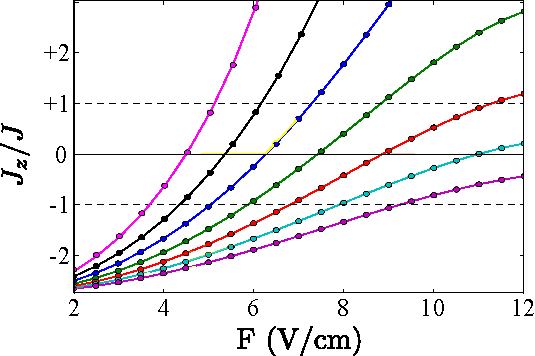
\includegraphics[width=0.7\linewidth]{figures/circsim/Jz_Jscan}
\caption[Variation de $J_z/J$]{
Variation de $J_z/J$ pour une paire d'atomes dans les niveaux $\ket{\mathrm{50C}}$ et $\ket{\mathrm{48C}}$, en fonction du champ électrique $F$.
Le champ électrique est dirigé selon $Oz$ et les atomes sont situés sur l'axe $Ox$.
Les points sont obtenus par diagonalisation du hamiltonien de paire complet pour différentes valeurs de champ magnétique $B_z=\SI{9}{},\SI{10}{},\SI{11}{},\SI{12}{},\SI{13}{},\SI{14}{}$ et $\SI{15}{\gauss}$, de gauche à droite (points de couleur magenta, noir, bleu, vert, rouge, cyan et violet respectivement).
Les lignes qui les relient sont des guides visuels.
}
\label{fig:Jz_Jscan}
\end{figure}

Quelle physique ? Diagramme de phase.
%
\begin{figure}[!h]
\centering
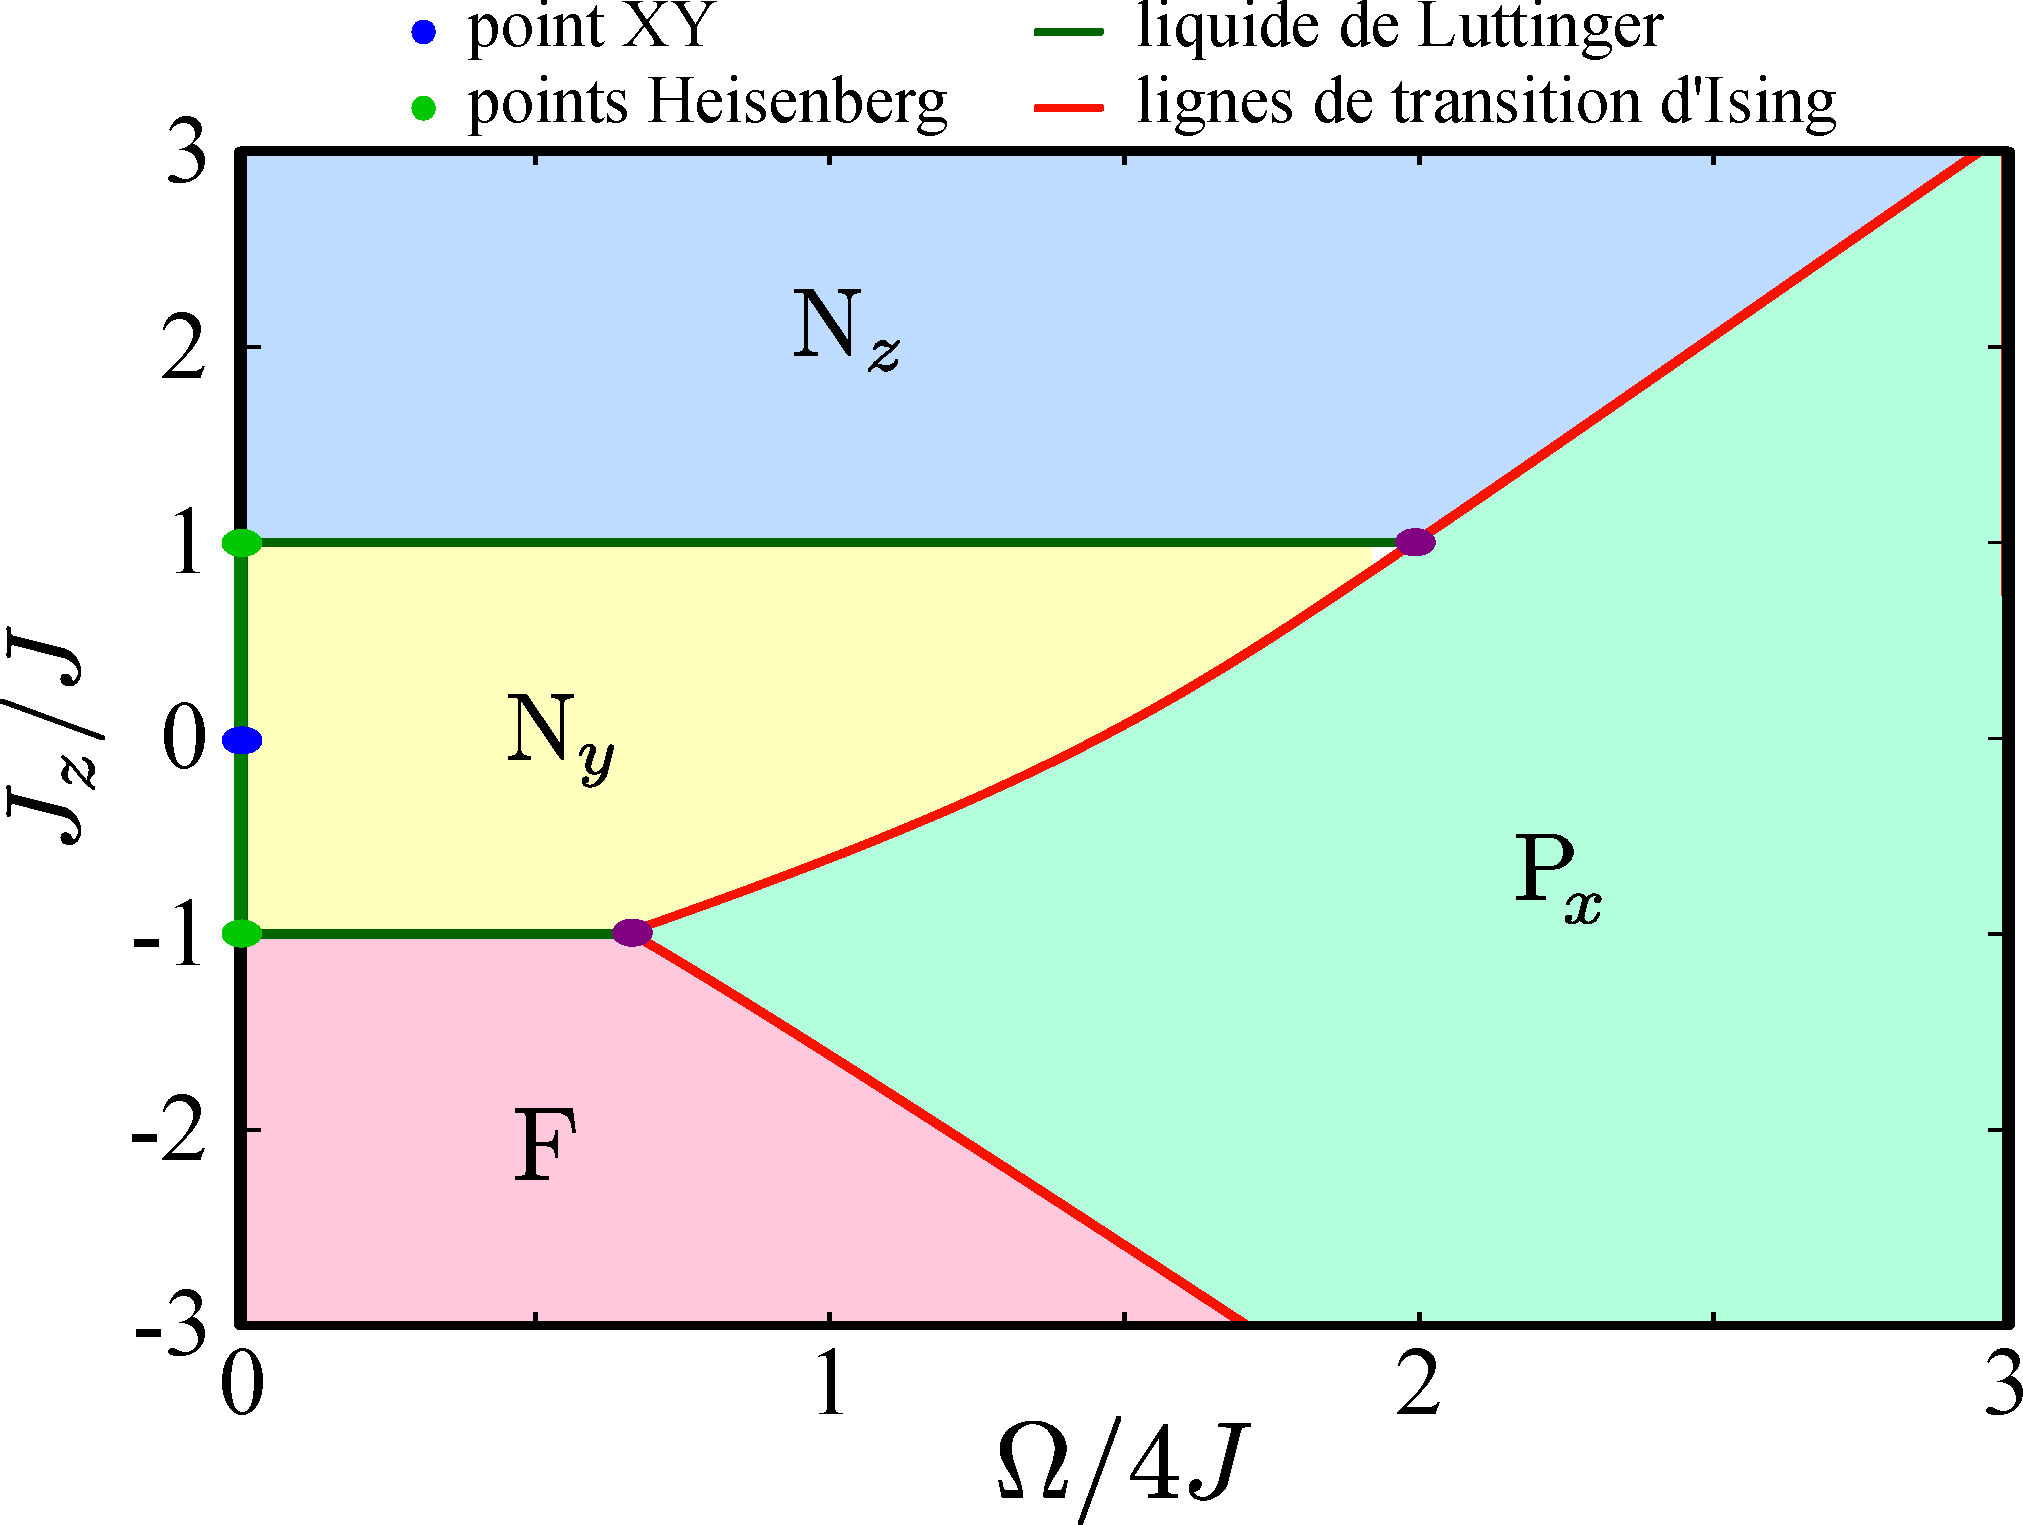
\includegraphics[width=0.7\linewidth]{figures/circsim/phase_diagram}
\caption[Diagramme de phase]{
Diagramme de phase.
}
\label{fig:phase_diagram}
\end{figure}

\newpage

\section{Principes techniques du simulateur}
	\subsection{Piégeage laser des Rydberg circulaires}
	\subsection{Préservation des états de Rydberg}\label{subsec:inhibition}
		\subsubsection*{Temps de vie dans l'espace libre}
		\subsubsection*{Inhibition de l'émission spontanée}
		\subsubsection*{Problème du mixing et solution}
	\subsection{Préparation déterministe d'une chaîne}

\newpage
Reprendre le PRX